\documentclass{article}
\usepackage[T1]{fontenc}
\usepackage{geometry}
\geometry{a4paper}
\usepackage{setspace}
\usepackage{enumerate}
\usepackage{enumitem}
\usepackage{hyperref}
\usepackage{parskip}
\usepackage[toc]{glossaries}
\hypersetup{colorlinks,allcolors=black,urlcolor=blue}

\setenumerate[1]{itemsep=0pt,partopsep=2pt,parsep=0pt ,topsep=2pt}
\setitemize[1]{itemsep=0pt,partopsep=2pt,parsep=0pt ,topsep=2pt}
\setenumerate[2]{itemsep=0pt,partopsep=2pt,parsep=0pt ,topsep=2pt}
\setitemize[2]{itemsep=0pt,partopsep=2pt,parsep=0pt ,topsep=2pt}
\setdescription{itemsep=0pt,partopsep=2pt,parsep=0pt ,topsep=2pt}

\usepackage{graphicx}
\usepackage{fontspec}

\defaultfontfeatures{%
    RawFeature={%
        % +swsh,
        +calt
    }%
}

\setmainfont{EB Garamond}

\usepackage{multicol}
\usepackage{float}

\usepackage{longtable}

\usepackage[semibold]{sourcecodepro}

\usepackage{xcolor}
\usepackage{minted}
\usemintedstyle{friendly}

\definecolor{bg}{rgb}{0.95,0.95,0.95}
\newcommand{\codeinline}[1]{
    \mintinline[bgcolor=bg, fontsize=\scriptsize]{text}{#1}
}


\usepackage{relsize}
\newcommand{\bigdataVs}[1]{
    \subsection{#1}
}

\newenvironment{console}{% Caution:
    \VerbatimEnvironment
    \begin{minted}[xleftmargin=2em,bgcolor=bg,fontsize=\small]{console}% Do NOT delete these comments
    }% Otherwise there will be error when compiling
    {%
    \end{minted}%
}

\newenvironment{json}{% Caution:
    \VerbatimEnvironment
    \begin{minted}[xleftmargin=0em,bgcolor=bg,fontsize=\scriptsize]{json}% Do NOT delete these comments
    }% Otherwise there will be error when compiling
    {%
    \end{minted}%
}
%-----------%

\title{NoSQL Write-up -- Dota2 Game Replay Analysis}
\author{
    Team name: PSG.LGD \\ \\
    Yichun Yan \\
    Ziwei Jiang \\
    Yifan Li \\
    Weiqi Wang
}
\date{\today}


\makeglossaries


\newglossaryentry{Ancient}
{
    name={Ancient},
    description={(also commonly refered to as Thrones, or Tree for Radiant's ancient and Throne for Dire's ancient, as legacy names from DotA) are massive structures found inside each faction's base and are the main objective. In order to win, the enemy team's Ancient must be destroyed, while the own one must be kept alive. Ancients are guarded by their two tier 4 towers. The Ancients are invulnerable until both of their tier 4 towers are destroyed.}
}
\newglossaryentry{MOBA}
{
    name={MOBA},
    description={also known as action real-time strategy (ARTS), is a subgenre of strategy video games that originated as a subgenre of real-time strategy in which each player controls a single character, usually on a map in an isometric perspective, as part of a team competing against another team of players.}
}
\newglossaryentry{professional matches}
{
    name={professional matches},
    description={Matches played two professional teams hosted officially by Valve.}
}
\newglossaryentry{public matches}
{
    name={public matches},
    description={Matches played by ten randomly chosen players, and the results won't influence Matchmaking Rating(MMR) of each player.}
}
\newglossaryentry{ranked matches}
{
    name={ranked matches},
    description={Matches played by ten randomly chosen players according to their Matchmaking Rating(MMR), and the results will influence the Matchmaking Rating of each player.}
}
\newglossaryentry{gold}
{
    name={gold},
    description={Gold is the currency used to buy items or instantly revive your hero. Gold can be earned from killing heroes, creeps, or buildings.}
}
\newglossaryentry{creeps}
{
    name={creeps},
    description={Creeps are basic units in Dota 2. Every unit which is not a hero, building, ward or courier is considered a creep. Creeps can belong to either faction, be neutral, or be player-controlled units. Unlike heroes, creeps do not gain experience and cannot level up. All of their stats are set values (though can still be altered by modifiers). Most creeps grant a set gold and experience bounty to heroes when killed.}
}
\newglossaryentry{XP}
{
    name={XP},
    description={A shorthand for experience. Experience is an element heroes can gather by killing enemy units, or being present as enemy units get killed. On its own, experience does nothing, but when accumulated, it increases the hero's level, so that they grow more powerful. Only heroes can gather experience and therefore reach higher levels. With each level gained, a hero's base attributes increase by static values (unique for each hero), which makes them stronger in several.}
}
\newglossaryentry{match id}
{
    name={match id},
    description={A unique identifier for each match played on Dota2.}
}
\newglossaryentry{sequence number}
{
    name={sequence number},
    description={Similar to match id, which is a unique identifier for each match. But this field will not show up in the Dota2's client.}
}
\newglossaryentry{towers}
{
    name={towers},
    description={Towers are the main line of defense for both teams, attacking any non-neutral enemy that gets within their range. Both factions have all three lanes guarded by three towers each.}
}
\newglossaryentry{barracks}
{
    name={barracks},
    description={Barracks (commonly shortened to Rax) are buildings, defended by their tier 3 towers, that are responsible for keeping lane creeps as powerful as their counterparts.}
}
\newglossaryentry{lane}
{
    name={lane},
    description={A Lane is one of three paths connecting the two Ancients. Lane creeps will push along these lanes after spawning.}
}
\newglossaryentry{AFK}
{
    name={AFK},
    description={A shorthand for away-from-keyboard, AFK means a player leaving a match early before it's end.}
}
\newglossaryentry{buff}
{
    name={buff},
    description={Buffs are positive status effects that enhance your hero.}
}
\newglossaryentry{debuff}
{
    name={debuff},
    description={Debuffs are negative status effects that weaken your hero.}
}
\newglossaryentry{mode}
{
    name={mode},
    description={Game modes are a set of restrictions within which the game of Dota 2 can be played. Most game modes alter how heroes are picked by players. There are also some novelty modes that allow 1v1 play, or give a player a new hero every time they die, for example. }
}
\newglossaryentry{ban}
{
    name={ban},
    description={A ban will disallow the choose for a specific hero within a match.}
}
\newglossaryentry{pick}
{
    name={pick},
    description={A pick is choosing a hero that a player want to play within a match.}
}
\newglossaryentry{first-blood}
{
    name={first-blood},
    description={The first kill within a game. The player who makes the first kill will be rewarded with 150 extra gold}.
}
\newglossaryentry{team battle}
{
    name={team battle},
    description={A battle involves more than half of the players in a match within a short period of time}.
}
\newglossaryentry{buyback}
{
    name={buyback},
    description={While dead, the player has the option to use ``buyback", spending money in order to instantly respawn at the fountain. However, the buyback ability has a long cooldown of 480 seconds and has a scaling gold cost.}.
}
\newglossaryentry{last-hit}
{
    name={last-hit},
    description={You can only get gold from killing creeps or get a kill from killing a hero if you make the last-hit that cause the creeps or hero to death.}.
}
\begin{document}

\maketitle

\tableofcontents
\clearpage

%-------%

\section{Datasets}

\subsection{Background of Datasets}

Our team aims at exploring data about a popular and long-lived computer game, Dota2.

Dota2 is a multiplayer online battle arena (\gls{MOBA}) video game developed and published by Valve Corporation. Each game will involve ten players that are divided to two teams play against each other on a same map. Every player chooses one ``hero" that has unique abilities and different styles of playing. The aim for each team is to destroy the building called ``\gls{Ancient}" of the other team. Players collect \gls{gold} to buy powerful items and gain \gls{XP} by killing players on the other team, destroy building of the other team, or kill \gls{creeps}.

\begin{figure}[H]
    \centering
    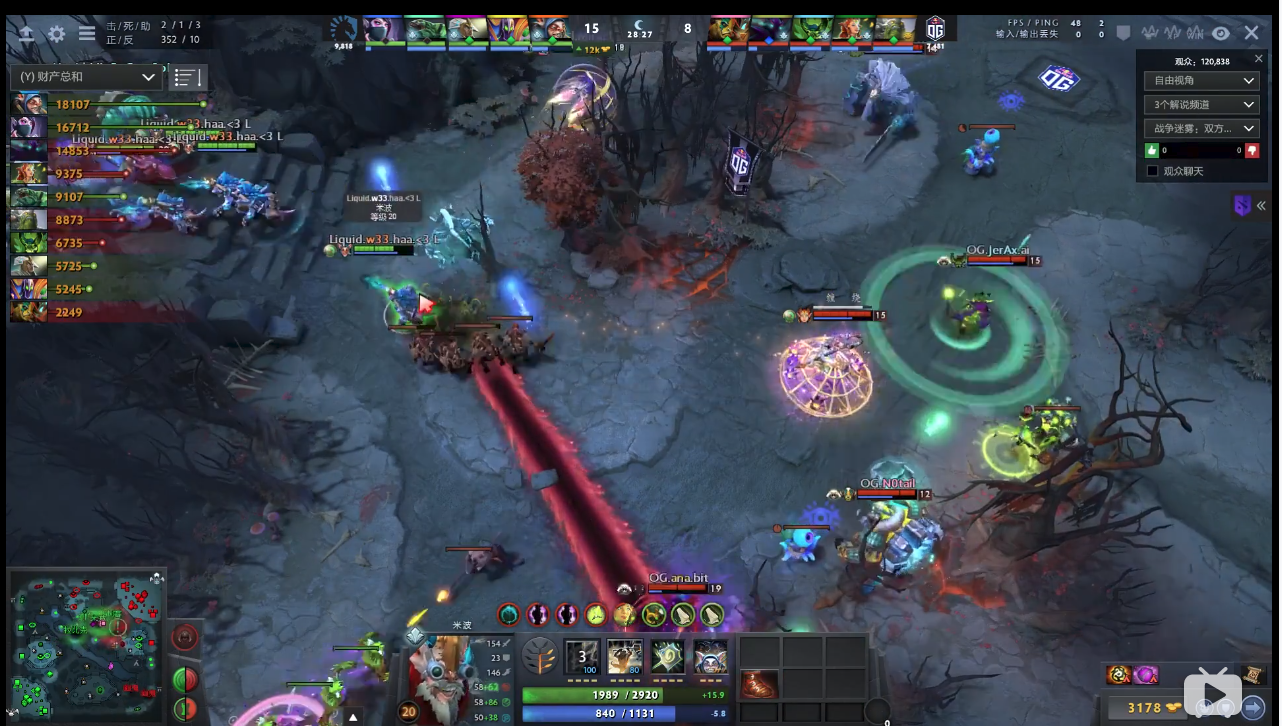
\includegraphics[width=\linewidth]{pic/combat.png}
    \caption{A screenshot of the game}
\end{figure}

This game has a large quantity of players, accordingly a huge amount of replays will be produced every day. Also, it's a real-time game, hundreds of operations and some decisions will be made each second, and all of them will have some influence on the final results of the game. Both of the above two features make the game a great subject to big data analysis.

Actually, there are some professional teams start hiring data engineers to help their players perform better in a game. This means that our analysis has some realistic meaning.
For example, by using big data pipeline to answer the business question "Does there exist a regular farming path for some professional players?", we can understand both our teammates and the opponents better, and therefore optimize our strategies.

We have used technologies like MongoDB, Apache Spark, Neo4j for this project. All of the code of this project can be found in \href{https://github.com/Vopaaz/big-data-psg-lgd/tree/a9a285e0e29c0d9e56b41994875df830c7e7b51b}{this repository}, and I will explain the logic of our project and reference to some lines of code when necessary in the following sections.

\subsection{Source of Datasets}

\renewcommand{\arraystretch}{1.5}
\begin{table}[H]
\centering
\begin{tabular}{lll}
    Dataset Name & Source & Format \\\hline

    \href{https://wiki.teamfortress.com/wiki/WebAPI/GetMatchDetails}{Dota2 match result dataset} &
    \href{https://wiki.teamfortress.com/wiki/WebAPI}{Valve's official API} &
    JSON file in \href{https://wiki.teamfortress.com/wiki/WebAPI/GetMatchDetails}{this schema}\\

    \href{https://wiki.teamfortress.com/wiki/Replay}{Dota2 replay dataset} &
    Valve's Dota2 replay servers \footnotemark &
    \renewcommand{\arraystretch}{1}
    \begin{tabular}{@{}l@{}}
    \codeinline{.dem} binary format, designed for\\ Dota2 game client and need to be parsed
    \end{tabular}
    \renewcommand{\arraystretch}{1.5}
\end{tabular}
\end{table}

\footnotetext{urls for downloading replay can be constructed by combining the information in \href{https://docs.opendota.com/}{an OpenDota API} and \href{https://wiki.teamfortress.com/wiki/WebAPI/GetMatchDetails}{one of the Valve's Official API}.}


\subsection{Descriptions of Datasets}

\begin{enumerate}
\item Dota2 match result dataset: Snapshot of the end of a game, including the winner team, the duration of the whole game, each player's ending level, items and kill/death/assist, and other important information about the game and each player.
\item Dota2 replay dataset: Everything happens in a game, which includes the whole combat log of the game, chatting information and the spawn and death of NPCs.
\end{enumerate}

We will discuss how we acquire those data how it is transformed into a usable format in details in the ETL selection.

\subsection{Data Dictionaries}

The Dota2 match result data is already in JSON format, we can use it straightforwardly in the same schema to save it into our database. The data dictionary for this dataset can be found in table \ref{match-result-data-dictionary}, \ref{player-field-in-match-result} and \ref{ban-pick-in-match-result} in the Appendix.

The replay dataset is initially binary files, therefore we have to parse it first then fit into a schema that we design. After these process, one document(record) of a replay should have the following fields:

\begin{longtable}{|p{2cm}|p{2cm}|p{4.5cm}|p{5cm}|}

\hline
\textbf{Field Name} & \textbf{Data Type} & \textbf{Description}  & \textbf{Example} \\
\hline
\endhead

match\_id & long & The unique match id of this match & 4986514901\\\hline
combatlog & JSON Array & Describing all the events in the game. See next table for details & See next table \\\hline
chat &  JSON Array & What the players say in the chat during the match &
\begin{minipage}{4.99cm}
\begin{json}
{
  "sender": "Sk SpwaN",
  "message": "gg wp"
}
\end{json}
\end{minipage}
\\\hline
lifestate & JSON Array & Spawns and deaths of objects in the game & 
\begin{minipage}{4.99cm}
\begin{json}
{
  "tick": 7420,
  "type": "spawn",
  "object":
    "CDOTA_BaseNPC_Creep_Lane"
}
\end{json}
\end{minipage}
\\\hline
\caption{Replay Data Dictionary}
\end{longtable}


The data dictionary for one JSON object of field "combatlog" that mentioned before should be: \\

\begin{tabular}{|p{3cm}|p{2cm}|p{5cm}|p{3cm}|}
\hline
Field Name& Data Type& Description & Example\\
\hline
time & double & The time when this action happens & 325.608734130432 \\
\hline
type & String & The type of this action. & "purchase" \\
\hline
target & String & The target of this action & "npc\_dota\_hero\_nevermore" \\
\hline
item & String & This field only occurs when the type of the action is "purchase". Indicates which item was bought by this action & "item\_enchanted\_mongo" \\
\hline
inflictor & String & This field only occurs when the type of the action is "damage", "lose\_buff" and "add\_buff". The inflictor of the current action & "modifier\_tower\_aura\_bonus" \\
\hline
damage & int & This field only occurs when the type of the action is "damage", which indicates the damage caused by the current action. & 80 \\
\hline
before\_hp & int &  This field only occurs when the type of the action is "damage", which indicates the hp of the target before the action. & 725 \\
\hline
after\_hp & int &  This field only occurs when the type of the action is "damage", which indicates the hp of the target after the action. & 718 \\
\hline
\end{tabular}

The more detailed data dictionary of field "info" that mentioned before should be: \\
\begin{tabular}{|p{3cm}|p{2cm}|p{5cm}|p{3cm}|}
\hline
Field Name& Data Type& Description & Example\\
\hline
game\_winner & int & 1 if radiant wins and 2 if dire wins. & 1 \\
\hline
leagueid & int & The unique league id of the current professional game, 0 if it is not a professional match. & 4122 \\
\hline
match\_id & long & The unique identifier for each game. & 4986514901. \\
\hline
end\_time & long & The timestamp of the ending of the game. & 1566736571. \\
\hline
game\_mode & int & The mode of the current game & 21 \\
\hline
\end{tabular}
\section{Data ETL}
Our aim is to collect about 1,500,000 records for our match result dataset and about 1000 professional games, 1000 ranked games and 1000 public games for our replay dataset. Our data is mainly three sources:
\begin{enumerate}
\item \href{https://wiki.teamfortress.com/wiki/WebAPI/}{Valve's official api}.
\item \href{https://docs.opendota.com/}{OpenDota's third party api}.
\item \href{https://dev.dota2.com/showthread.php?t=47115}{Dota2's replay cluster}.
\end{enumerate}
    I will walk through how I create a pipeline to make use of the above three sources to collect all the data I want in the Extraction section. \\
\subsection{Extraction}

    First, in order to call the Valve's official api, we need a key to get authorized. To avoid the api call limits of the api, I create a key pool that contains 5 different authorizing keys that are obtained using our steam accounts. Every time I need to call the api I just randomly \href{https://github.com/Vopaaz/big-data-psg-lgd/blob/a9a285e0e29c0d9e56b41994875df830c7e7b51b/src/main/java/FetchStore/ValveAPI.java#L215}{pick one key from the poll}. Tha api we are mainly using is \href{https://wiki.teamfortress.com/wiki/WebAPI/GetMatchHistoryBySequenceNum}{this one}. Which requires two parameters: \codeinline{start_at_match_seq_num} and \codeinline{matches_requested}.
The first one is an unique identifier for each match, and the api will return a number of results that equals to the second parameter you give to the api in \href{https://wiki.teamfortress.com/wiki/WebAPI/GetMatchDetails}{this JSON format}. We construct the url for the api call \href{https://github.com/Vopaaz/big-data-psg-lgd/blob/a9a285e0e29c0d9e56b41994875df830c7e7b51b/src/main/java/FetchStore/ValveAPI.java#L207-L230}{like this} to get a bunch of match results and \href{https://github.com/Vopaaz/big-data-psg-lgd/blob/a9a285e0e29c0d9e56b41994875df830c7e7b51b/src/main/java/FetchStore/ValveAPI.java#L238-L257}{save them into MongoDB}. Also, since we always want to keep the HiFi data around, I also \href{https://github.com/Vopaaz/big-data-psg-lgd/blob/a9a285e0e29c0d9e56b41994875df830c7e7b51b/src/main/java/FetchStore/ValveAPI.java#L289-L300}{wrote the original JSON file into the disk}. After we get a list of match result in the previous call, we can use the sequence number of the last record we get from the last call then \href{https://github.com/Vopaaz/big-data-psg-lgd/blob/a9a285e0e29c0d9e56b41994875df830c7e7b51b/src/main/java/FetchStore/ValveAPI.java#L275}{plus one} as the \codeinline{start_at_match_seq_num} for the next iteration. Also, considering the ratio of professional games is very small, I iterate the whole results to find out whether there is a \href{https://github.com/Vopaaz/big-data-psg-lgd/blob/a9a285e0e29c0d9e56b41994875df830c7e7b51b/src/main/java/FetchStore/ValveAPI.java#L146-L161}{valid} professional game. If I find a valid professional game, I will call \href{https://docs.opendota.com}{OpenDota's API} using the \codeinline{match_id}, which is also an unique identifier of the professional game and can be obtained by the previous results to get the information we need to download the replays. Then we use this information to \href{https://github.com/Vopaaz/big-data-psg-lgd/blob/a9a285e0e29c0d9e56b41994875df830c7e7b51b/src/main/java/FetchStore/OpendotaAPI.java#L17-L70}{construct an url} like this format \codeinline{http://replay<cluster>.valve.net/570/<match_id>_<replay_salt>.dem.bz2} and \href{https://github.com/Vopaaz/big-data-psg-lgd/blob/a9a285e0e29c0d9e56b41994875df830c7e7b51b/src/main/java/FetchStore/ValveAPI.java#L131-L144}{start another thread} to to \href{https://github.com/Vopaaz/big-data-psg-lgd/blob/a9a285e0e29c0d9e56b41994875df830c7e7b51b/src/main/java/FetchStore/ValveAPI.java#L389-L420}{download, unzip and parse the replay}. At the same time, since we want to get a same number of ranked matches and public matches, we maintain \href{https://github.com/Vopaaz/big-data-psg-lgd/blob/a9a285e0e29c0d9e56b41994875df830c7e7b51b/src/main/java/FetchStore/ValveAPI.java#L46-L47}{two integers} to record how many public matches and ranked matches to download. As we start downloading a professional match, we \href{https://github.com/Vopaaz/big-data-psg-lgd/blob/a9a285e0e29c0d9e56b41994875df830c7e7b51b/src/main/java/FetchStore/ValveAPI.java#L111-L112}{add one} to those two integers, and if the numbers are not zero when we encounter a public match result or a ranked match, we start to download them using the same method I used for professional games, this logic can be mapped to \href{https://github.com/Vopaaz/big-data-psg-lgd/blob/a9a285e0e29c0d9e56b41994875df830c7e7b51b/src/main/java/FetchStore/ValveAPI.java#L104-L129}{this snippet of code}. This way we can get game replays of three types in same amount for the second dataset while we collect the data for the first dataset.
\subsection{Transformation}
    The match result dataset is easy to handle, since the result of  \href{https://wiki.teamfortress.com/wiki/WebAPI/GetMatchHistoryBySequenceNum}{this api} is just a JSON string, which can be easily \href{https://github.com/Vopaaz/big-data-psg-lgd/blob/9916e0a5a95245062d110446eb4014312087ef9e/src/main/java/FetchStore/ValveAPI.java#L164-L178}{parsed into Document} datatype by the MongoDB Driver in Java and saved to MongoDB. But the replay is in binary format, which can only be executed by the Dota2's client. We need to use some open-source parser to help us transform it into something that makes more sense to us. Luckily, we found \href{https://github.com/skadistats/clarity}{this parser} on GitHub. When use the pipeline that mentioned before to download and unzip each replay and parse it into strings, then use the schema we mentioned in the Data Dictionaries section. The code to parse the strings into our schema is following:
\begin{enumerate}
\item \href{https://github.com/Vopaaz/big-data-psg-lgd/blob/master/src/main/java/ParseReplay/ParseReplayExecutor.java}{The overall logic}.
\item \href{https://github.com/Vopaaz/big-data-psg-lgd/blob/master/src/main/java/ParseReplay/Info.java}{For the "info" field}.
\item \href{https://github.com/Vopaaz/big-data-psg-lgd/blob/master/src/main/java/ParseReplay/Combatlog.java}{For the "combatlog" field }.
\item \href{https://github.com/Vopaaz/big-data-psg-lgd/blob/master/src/main/java/ParseReplay/Chat.java}{For the "chat" field}.
\item \href{https://github.com/Vopaaz/big-data-psg-lgd/blob/master/src/main/java/ParseReplay/Lifestate.java}{For the "lifestate" field}.
\end{enumerate}

\subsection{Loading}
We deploy our database on AWS EC2, I used \href{https://github.com/Vopaaz/big-data-psg-lgd/blob/a9a285e0e29c0d9e56b41994875df830c7e7b51b/src/main/java/FetchStore/ValveAPI.java#L164-L178}{this snippet} of code to save the JSON format match result data into MongoDB and \href{https://github.com/Vopaaz/big-data-psg-lgd/blob/a9a285e0e29c0d9e56b41994875df830c7e7b51b/src/main/java/FetchStore/ValveAPI.java#L406-L420}{this snippet} of code to write parsed replay data into MongoDB.
The size of our dataset: \\

\begin{tabular}{|c|c|c|}
\hline
Dataset Name & Number of records & Storage Size \\
\hline
Dota2 match result & About 1,500,000 & About 15 GB \\
\hline
Dota2 replay dataset & About 3500 & About 35 GB \\
\hline
\end{tabular}

\section{Data Analysis}
In data analysis we used Neo4j to analyze the win-lose relationship between professional games. And use Spark to analyze business questions raised in our proposal. We don't fulfill all business questions and we will state the reason for it in the challenges section. We have 3 game types: the public game, the ranked game, the professional game. Most following business questions are answered in these three game types. So we have the first step to \href{https://github.com/Vopaaz/big-data-psg-lgd/blob/master/src/main/scala/Spark/SparkMongoHelper.scala#L31-L47}{filter games by their types}. Here are business questions we completed:
\begin{enumerate}
    \item Bad Manner \\
    This analysis is aimed to find out the hero which has the most possibility to be a bad manner player. We define a bad manner as leaving a game before the game ends. We use match result data, since it contains leave game statu. We do \href{https://github.com/Vopaaz/big-data-psg-lgd/blob/master/src/main/scala/BadManner.scala#L46-L47}{aggregation on the hero id to get the pairs of a hero id and a leave game count}. Before further steps, we first check if there is no bad manner player, which turns out to be true in professional games. Then for each pair, we \href{https://github.com/Vopaaz/big-data-psg-lgd/blob/master/src/main/scala/BadManner.scala#L48}{divide the leave game count by the total pick count of this hero to compute the possibility}. Finally, we can get the bad manner hero by \href{https://github.com/Vopaaz/big-data-psg-lgd/blob/master/src/main/scala/BadManner.scala#L50}{sorting the processed pairs}. In public games, hero which has the most possibility to be a bad manner player is Broodmother, who has 10\% leave game rate. In ranked games, it is Meepo, who has 5\% leave rate. And in professional games, there are almost no players leave a game before a game ends. Through the result, we can find out that players are more serious in ranked games than the public, since ranked games affect their rankings.
    \item Cost Time \\
    This analysis is aimed to find out the average cost time. We use the match result data which has the game duration. For each match result data, we can \href{https://github.com/Vopaaz/big-data-psg-lgd/blob/master/src/main/scala/CostTime.scala#L30}{extract the duration and increment the total game count by 1}. Finally, we can get the average cost of time by \href{https://github.com/Vopaaz/big-data-psg-lgd/blob/master/src/main/scala/CostTime.scala#L31}{dividing the sum of all duration by the total game count}. For public games, the average cost of time is 33 minutes. For ranked games, the average time is 40 minutes. For professional game, the average time is 30 minutes.
    \item Damage Rate \\
    This analysis is aimed to find out the heroes who have the top 20 damage rate and the heroes who have the bottom 20 damage rate. We define the damage rate of a hero as the damage to other heroes per gold gained by the hero. We use match result data which contains damage to other heroes, gold spent, and rest gold of each hero. For each match result, we \href{https://github.com/Vopaaz/big-data-psg-lgd/blob/master/src/main/scala/DamageRate.scala#L39-L41}{extract the 3tuple of a hero id, a total damage to other heroes, a total gained gold (addition of gold spend and rest gold)}. Then we do \href{https://github.com/Vopaaz/big-data-psg-lgd/blob/master/src/main/scala/DamageRate.scala#L42-L44}{an aggregation on the hero id and divide the damage by the gained gold to get pairs of a hero id and a damage rate}. Finally, to get the top 20 heroes and the bottom 20 heroes, we can simply \href{https://github.com/Vopaaz/big-data-psg-lgd/blob/master/src/main/scala/DamageRate.scala#L47-L48}{sort pairs by the damage rate}. We list the result for this analysis in the Appendix.
    \item Economy Distribution vs Game Result \\
    This analysis is aimed to find out whether there exists a correlation between economy distribution in a game and the game result. We define the economy as gold gained in a game, since it's limited in a game, we hypothesize that the distribution of gold affects on the game result. It's possible that even distribution is better and it's also possible that good players gaining more gold is better. To exam the hypothesis, we \href{https://github.com/Vopaaz/big-data-psg-lgd/blob/master/src/main/scala/EcoDistributionTrain.scala#L48-L50}{apply logistic regression} in this analysis. We use the match result data which contains the amount of gold gained per minute for each player. For each match result data, we \href{https://github.com/Vopaaz/big-data-psg-lgd/blob/master/src/main/scala/EcoDistributionTrain.scala#L36-L42}{extract a pair of a game result, a normalized gold distribution}. A gold distribution contains the proportion of gold of 5 players in a game. For each distribution, we \href{https://github.com/Vopaaz/big-data-psg-lgd/blob/master/src/main/scala/EcoDistributionTrain.scala#L43-L44}{sort it in ascending order} to make the smallest proportion at the head of the distribution. Then we can use sorted distribution as the data point for the logistic regression model. Each proportion of distribution is a feature. And we use the game result as the label for logistic regression. After running the training data, we find the accuracy is only 0.53 which is close to making a guess. Thus, our hypothesis turns out to be false.
    \item Gain in First 15 Minutes \\
    This analysis is aimed to find out the hero who gains most XP or gold. We use replay data which contains all events during a game. We first \href{https://github.com/Vopaaz/big-data-psg-lgd/blob/master/src/main/scala/First15minGain.scala#L44-L47}{filter by XP or gold}. We can extract the time when this event happened. Thus, we can filter events to \href{https://github.com/Vopaaz/big-data-psg-lgd/blob/master/src/main/scala/First15minGain.scala#L48-L50}{get only the first 15 minutes events of gaining XP/gold}. Then we can \href{https://github.com/Vopaaz/big-data-psg-lgd/blob/master/src/main/scala/First15minGain.scala#L81-L82}{do aggregation on hero name} to calculate the total gain XP/gold. Finally, we \href{https://github.com/Vopaaz/big-data-psg-lgd/blob/master/src/main/scala/First15minGain.scala#L89-L96}{sort the gained XP/gold value} to compute the hero who gains most XP/gold in 3 game types. We list the result for this analysis in the Appendix.
    \item First Blood vs Cost Time\\
    This analysis is aimed to find out the correlation between the time of first blood and the total cost of time in a game. The first blood is the first kill in a game. We guess early first blood means a game is fast. To exam our guess, we \href{https://github.com/Vopaaz/big-data-psg-lgd/blob/master/src/main/scala/FirstBloodTrain.scala#L31-L33}{apply linear regression} in this analysis. We use match result data which contains the first blood time and the total duration. For each match result, we extract the first blood time and the game result. The data point used in linear regression is the time of the first blood. The label used is the game result. But the root mean squared error on training data is 765 which is large. The error shows that there is no correlation between the first blood time and the cost of time.
    \item Most Stats Hero \\
    This analysis is aimed to find out the top 5 heroes who have most kills/assists/deaths/heals. We use replay data which contains all events during a game. We first \href{https://github.com/Vopaaz/big-data-psg-lgd/blob/master/src/main/scala/HeroMostStats.scala#L60}{filter by the event type we want (kill/assist/death/heal)}. Then for each replay data, we \href{https://github.com/Vopaaz/big-data-psg-lgd/blob/master/src/main/scala/HeroMostStats.scala#L61}{extract a pair of a hero id and a count of the event type}. Then we \href{https://github.com/Vopaaz/big-data-psg-lgd/blob/master/src/main/scala/HeroMostStats.scala#L62}{do aggregation} on the hero id and \href{https://github.com/Vopaaz/big-data-psg-lgd/blob/master/src/main/scala/HeroMostStats.scala#L65}{sort pairs} by the count to extract the top 5 heroes. We list the result for this analysis in the Appendix.
    \item Most Ban \\
    This analysis is aimed to find out the top 5 heroes who are banned in professional games (only professional game allows banning heroes). We use match result data which contains banned heroes. We first filter games to keep only professional games. Then we \href{https://github.com/Vopaaz/big-data-psg-lgd/blob/master/src/main/scala/MostBan.scala#L29-L30}{extract a pair of a hero id and 1 (denotes banned once) for each match result data}. After \href{https://github.com/Vopaaz/big-data-psg-lgd/blob/master/src/main/scala/MostBan.scala#L31}{doing aggregation} on the hero id, we \href{https://github.com/Vopaaz/big-data-psg-lgd/blob/master/src/main/scala/MostBan.scala#L33}{sort the banned count} to get the top 5 banned heroes. They are Alchemist, Enchantress, Shadow Demon, Faceless Void, and Life Stealer. And we can find some of them has a good ranking in the previous analysis. For example, Alchemist has a 7th damage rate in public games.
    \item Most Pick \\
    This analysis is aimed to find out the top 5 heroes who are picked. We use match result data which contains picked heroes of each game. We \href{https://github.com/Vopaaz/big-data-psg-lgd/blob/master/src/main/scala/MostPick.scala#L34}{extract pairs of a hero id and 1 (denotes picked once)}. After \href{https://github.com/Vopaaz/big-data-psg-lgd/blob/master/src/main/scala/MostPick.scala#L35}{doing aggregation} on the hero id, we \href{https://github.com/Vopaaz/big-data-psg-lgd/blob/master/src/main/scala/MostPick.scala#L37}{sort the picked count} to get the top 5 picked heroes. We list the result for this analysis in the Appendix.
    \item Most Used/Purchased Item \\
    These two analysis are aimed to find out the top 5 most used/purchased items. We use replay data in this analysis because it contains all events happen during a game. In Most Used Item analysis, we \href{https://github.com/Vopaaz/big-data-psg-lgd/blob/master/src/main/scala/MostUsedItem.scala#L38-L40}{filter events contained in replay data to get all 'use item' events}. Then we \href{https://github.com/Vopaaz/big-data-psg-lgd/blob/master/src/main/scala/MostUsedItem.scala#L41-L42}{do aggregation on the item id} to get the pairs of an item id and an item use count. Finally, we can get the top 5 most used items by \href{https://github.com/Vopaaz/big-data-psg-lgd/blob/master/src/main/scala/MostUsedItem.scala#L44}{sorting the pairs by the use count}. We have similar steps in \href{https://github.com/Vopaaz/big-data-psg-lgd/blob/master/src/main/scala/MostPurchasedItem.scala}{Most Purchased Item} analysis. We list the result for this analysis in the Appendix.
    \item Team Battle Detector\\
    This analysis aimed to find out the average first time a team battle and the average times of team battle happens in public, ranked, and professional games. We use the replay data which has all events. But these events don't have the location of events. Thus, we roughly define the team battle as in 3 minutes there are 4 or more hero deaths. We apply \href{https://github.com/Vopaaz/big-data-psg-lgd/blob/master/src/main/scala/TeamBattleDetector.scala#L61-L78}{a sliding-window algorithm} to build a team battle detector. We \href{https://github.com/Vopaaz/big-data-psg-lgd/blob/master/src/main/scala/TeamBattleDetector.scala#L33-L36}{extract the death events} and use the detector to detect all team battles in a game. The time of the first team battle is at 11 minutes, 13 minutes and 19 minutes in public, ranked, and professional game. The average number of team battles is 7, 9, and 6 in public, ranked, and professional game respectively.
\end{enumerate}
Additionally, for most analysis above, we can only get the hero id or item id. To provide better readability, we add two metadata collection heros and items which contain hero/item ids and their names. So after getting the id, we do one more \href{https://github.com/Vopaaz/big-data-psg-lgd/blob/master/src/main/scala/Spark/SparkMongoHelper.scala#L15-L29}{query on the matadata collections to get the its name}.
\section{Challenges}
I will walk through the challenges we met during this project in the following subsections.
\subsection{Valve API}
Valve provides us with various apis to get match results, but they're not well documented and changes all the time without documentation. At the beginning I tried to use this \href{https://wiki.teamfortress.com/wiki/WebAPI/GetMatchHistory}{api}, which is very straightforward. This api requires us to specify a starting match ID and collect a bunch of match results starting with that match ID. But unfortunately I couldn't use it now since Valve didn't allow us to specify such an ID and it can just return the newest results that are currently produced, and it was never documented. I have thought that I could use this \href{https://wiki.teamfortress.com/wiki/WebAPI/GetMatchHistory}{api} to make a data stream for stream analysis, but this couldn't be done to since Valve limited its api calling gap. It's said to be 100,000 calls per day but actually you can do much less. I set the api calling interval to 6 seconds and sometimes it still denies the calls. Considering the velocity that the game results are produced we can't make such a stream to catch all the game results that are being produced. After exploring the Dota2 developers' forum for a while, I found out that we can use this  \href{https://wiki.teamfortress.com/wiki/WebAPI/GetMatchHistoryBySequenceNum}{api}, which works similarly as the before one but this time we need to specify a starting sequence number, which is also a unique identifier for each game but we can't see it in the Dota2's client so it gives us more difficulty. Later I found out that I can find the sequence number in this \href{https://wiki.teamfortress.com/wiki/WebAPI/GetMatchHistoryBySequenceNum}{website}. So I can first choose a starting sequence number by looking for a sequence number of a match whose date is around the starting date of all the matches I want to collect.  By calling this \href{https://wiki.teamfortress.com/wiki/WebAPI/GetMatchHistoryBySequenceNum}{api}, we can get a bunch of match results, so we can extract the sequence number of the last match of the results and plus 1 to it as the starting sequence number of the next request to the api. By doing this repeatedly, we can collect as many matches we want. As I mentioned, the api call limits are much less than it is described and it seems to be random. I created a request key pool to randomly select a key for the api call each time and if I was denied, I \href{https://github.com/Vopaaz/big-data-psg-lgd/blob/a9a285e0e29c0d9e56b41994875df830c7e7b51b/src/main/java/FetchStore/ValveAPI.java#L241-L249}{waited 3 seconds} then do the next call.
\subsection{Dota2 replays}
The replay dataset can be constructed by using url like this format: \\
\codeinline{http://replay<cluster>.valve.net/570/<matchid><replaysalt>.dem.bz2}. In the past, by calling this \href{https://wiki.teamfortress.com/wiki/WebAPI/GetMatchDetails}{api} using match ID of a game to get the cluster number and "replay salt" for a specific match. But now Valve disallowed us to do this too by hiding the "replay salt" field it the result due to the pressure on it's replay clusters is too large. Fortunately, I found another \href{third-party api}{https://docs.opendota.com/} that can help me find the fields I need to download a replay. So I thought of purely rely on this api to get the data in the first dataset, this way I can only use one kind of api to simplify the data pipeline. But this can't be done too, this third party api will ask us to pay if our request exceeds a certain number, that will cause cost exceeding our budget(which is zero). Also, we don't want to collect all the replays. It's clear that the matches played by the professional teams worth more than the normal ones. Given the limited time and storage we have, I think I will first collect a certain number of professional games, then collect public games and ranked games of the same number for comparing analysis with the professional games.

\subsection{Docker}

As mentioned in the proposal, we tried to containerized the project by docker, but it ends up with failures. Considering to the limited time, we decided to discard using docker for installing our NoSQL technology.

At first, I tried to dockerize our project by using a single Dockerfile. According to the \href{https://docs.docker.com/}{docker documents}, Dockerfile "defines what is going on in the environment inside your container". At the very beginning, I thought dockerize a project just need to pull all the official images in docker, and then we can start manipulate it. But then, after reading documents, I found that we need to construct a Dockerfile to define how a project work, so that it can behaves exactly the same wherever it runs. We can pull an image as a parent image, and then install needed packages in it.

For example, in the project, I used ubuntu as a parent image, then docker virtualized an ubuntu operation system environment on our host machine, and then I used Dockerfile as if it is the terminal of ubuntu, writing codes of installing java8, maven, mongodb in the Dockerfile.

After I constructed the Dockerfile, I failed every time when it was trying to connect to the database. Realized that it is cramped to put all the services on a Dockerfile, I tried to construct a docker-compose.yml to define, run and scale services with Docker.

According to our data pipeline, I intended to build 4 services in the docker-compose:
    \begin{itemize}
        \item Data acquisition and filtering (as "fetchstore" service in the docker-compose)
        \item Data Extraction (as "parsereplay" service in the docker-compose)
        \item Data Aggregation and Representation (as "mongodb" service in the docker-compose)
        \item Data Analysis (as "analytics" service in the docker-compose)
    \end{itemize}

In the docker-compose, we can also use the Dockerfile by using the command \codeinline{build} in a service. Therefore, I constructed Dockerfiles for Extraction, Transformation and Analysis services. And I used the official image of mongodb, and used \codeinline{volume} in the service to reflect the direction of configuration file and mongodb initial javascipt. Also, we used \codeinline{depends_on} to define simple interaction between the services.

As the result, we still have a hard time connecting the database. There are a lot of things to be considered when running multiple containers. When this problem is fixed, we only finished the configuration of the extraction and database service. Then we realized we got limited time left, therefore, we discard docker for now, and move on to deploy our project on amazon web service (AWS). And we hope to complete this part in the future.

The reason of failure is that I got misunderstanding on Docker's architecture. Also, it is hard for me to consider our system's architecture in Docker's way. Also it is time consuming to try those failures to realize the right way to deploy a project on Docker. This experience pushed me to learn a lot about Linux and to read a lot of configuration file.

\subsection{Setup AWS environment}
Because we planned to use over 200GB data, we decided to use AWS EC2 to run our system. We chose EBS (Elastic Block Store) which we thought would automatically have larger storage when our instance is full. But during fetching data, we still met the error which said the file system is full. Then we manually added more storage volume to solve this problem.
\subsection{Result Readability}
We have 2 types of data. But in match result data, the heroes and items inside are denoted by their id. But in replay data, they are denoted by their name. Obviously, using a name can increase readability. Thus, we added 2 more metadata collections to store the map from id to name.
\subsection{Corrupted Data}
Although we did some data validation before using it, there are still some unexpected corrupted data problems. For example, one replay data loses part of it which makes out result bad. So we added more filters in analysis, like the filter to the duration of a game.
\subsection{Setup Neo4j on AWS}
We want to setup Neo4j server on AWS and can be connected by a Neo4j browser on a local laptop. But the find the connection was failed. We first modified the configuration file of Neo4j which doesn't allow remote access in default. But the connection was still failed. Then we found out that we should modify the security group setting on AWS which controls access to the AWS instance.
\subsection{Miss Output on Console}
Firstly, we just printed the result on the console. But after we used our system on AWS, we found a problem that the connection from local to AWS might be broken. If so, we cannot get the result printed on the console. Thus, besides printing result on the console, we also write the result to a file, which prevents missing the output on the console.

\printglossary
%-------%

\section{Appendix}

\subsection{Detailed Data Dictionaries}

\subsubsection{Match Result Dataset}

\begin{longtable}{|p{3cm}|p{2cm}|p{5cm}|p{3cm}|}

\hline
\textbf{Field Name} & \textbf{Data Type} & \textbf{Description}  & \textbf{Example}\\
\hline
\endhead

players & JSON Array  & Status about each player at the end of the game, see next table for details & See next table.
\\
\hline
radiant\_win & boolean  & Dictates the winner of the match, true for radiant; false for dire. &true \\
\hline
duration  & int  & The length of the match, in seconds since the match began.  & 2452 \\
\hline
start\_time  & long  & Unix timestamp of when the match began.  & 1566731204 \\
\hline
match\_id  & long  & The matches unique ID.  & 4986382845 \\
\hline
match\_seq\_num  & long  & A `sequence number', representing the order in which matches were recorded.  & 4182489897 \\
\hline
tower\_status\_radiant and tower\_status\_dire  & int  & check \href{https://wiki.teamfortress.com/wiki/WebAPI/GetMatchDetails\#Tower\_Status}{this} for details.  & 260 \\
\hline
barracks\_status\_radiant and barracks\_status\_dire  & int  & check \href{https://wiki.teamfortress.com/wiki/WebAPI/GetMatchDetails\#Barracks\_Status}{this} for details. & 51 \\
\hline
first\_blood\_time  & int  & The time in seconds since the match began when first-blood occurred.  & 102 \\
\hline
lobby\_type  & int  & The type of the match  & 0 \\
\hline
human\_players  & int  & The amount of human players within the match.  & 10 \\
\hline
leagueid  & int  & The league that this match was a part of. A list of league IDs can be found via the \href{https://wiki.teamfortress.com/wiki/WebAPI/GetLeagueListing}{GetLeagueListing} method.
  & 0 \\
\hline
positive\_votes  & int  & The number of thumbs-up the game has received by users.  & 0 \\
\hline
negative\_votes  & int  & The number of thumbs-down the game has received by users.  & 1 \\
\hline
game\_mode  & int  & The mode of the match  & 11 \\
\hline
picks\_bans  & JSON Array  & A list of the picks and bans in the match, if the game mode is Captains Mode.  & Details will be described in another table \\
\hline
radiant\_score  & int  & The total amount of kills that radiant team make  & 52 \\
\hline
dire\_score  & int  & The total amount of kills that dire team make  & 42 \\
\hline
\caption{Match Result Data Dictionary}
\end{longtable}
\label{match-result-data-dictionary}


The data dictionary for one JSON object of field "players" in table \ref{match-result-data-dictionary} is as follows.

\begin{longtable}{|p{3cm}|p{2cm}|p{5cm}|p{3cm}|}

\hline
\textbf{Field Name} & \textbf{Data Type} & \textbf{Description}  & \textbf{Example} \\
\hline
\endhead

account\_id & long & An unique identifier for each steam account & 4294967295 \\
\hline
player\_slot & int & see this in details https://wiki.teamfortress.com/wiki/WebAPI/GetMatchDetails\#Player\_Slot & 1 \\
\hline
hero\_id & int & The hero's unique ID. A list of hero IDs can be found via the \href{https://wiki.teamfortress.com/wiki/WebAPI/GetHeroes}{GetHeroes} method. & 97 \\
\hline
item\_0 to item\_5 & int & item id of the inventory item & 48 \\
\hline
kills & int & The amount of kills attributed to this player. & 10 \\
\hline
deaths & int & The amount of times this player died during the match. & 2 \\
\hline
assists & int & The amount of assists attributed to this player. & 7 \\
\hline
leaver\_status & int & Indicating whether a player disconnect from the game before the game ends & 0 \\
\hline
gold & int & The amount of gold the player had remaining at the end of the match. & 32341 \\
\hline
last\_hits & int & The amount of last-hits the player got during the match. & 109 \\
\hline
denies & int & The amount of denies the player got during the match. & 24 \\
\hline
gold\_per\_min & int &  The player's overall gold/minute. & 601 \\
\hline
xp\_per\_min & int & The player's overall experience/minute. & 587 \\
\hline
gold\_spent & int & The amount of gold the player spent during the match. & 21239 \\
\hline
hero\_damage & int & The amount of damage the player dealt to heroes. & 34034 \\
\hline
tower\_damage & int & The amount of damage the player dealt to towers. & 8902 \\
\hline
hero\_healing & int & The amount of health the player had healed on heroes. & 452 \\
\hline
level & int & The player's level at match end. & 23 \\
\hline
\caption{Player Field in Match Result}
\end{longtable}
\label{player-field-in-match-result}


The data dictionary for one JSON object of field "picks\_bans" in table \ref{match-result-data-dictionary} is as follows.

\begin{longtable}{|p{3cm}|p{2cm}|p{5cm}|p{3cm}|}

\hline
\textbf{Field Name} & \textbf{Data Type} & \textbf{Description}  & \textbf{Example} \\
\hline
\endhead

is\_pick & boolean & Whether this entry is a pick (true) or a ban (false). & true \\
\hline
hero\_id & int & The hero's unique ID. & 20 \\
\hline
team & int & The team who chose the pick or ban; 0 for Radiant, 1 for Dire. & 1 \\
\hline
order & int & The order of which the picks and bans were selected. & 10 \\
\hline
\caption{Ban\_pick Field in Match Result}
\end{longtable}
\label{ban-pick-in-match-result}

\subsubsection{Parsed Replay Dataset}


\end{document}
